\documentclass[a4paper]{article}
\usepackage[cm]{fullpage}
\usepackage{standalone}
\usepackage[utf8]{inputenc}
\usepackage[british]{babel}
\usepackage{csquotes}
\usepackage[T1]{fontenc}
\usepackage{charter}
\usepackage[bitstream-charter]{mathdesign}
\usepackage{natbib}
\usepackage[final,babel]{microtype}
\usepackage[hidelinks]{hyperref}
\usepackage{siunitx}
\usepackage[margin=3pt]{subcaption}
\usepackage{xcolor}
\PassOptionsToPackage{final}{graphicx}
\usepackage{tikz}
\usetikzlibrary{arrows}
\usetikzlibrary{patterns}

\title{Monitoring Committee Progress Report \#1\\
\vspace*{1em}
\Large{Numerical Representation of Mountains in Atmospheric Models}}
\author{James Shaw
\vspace{0.5em} \\
\large{Supervisors: Hilary Weller, John Methven, Terry Davies}
\vspace{0.5em} \\
\large{Monitoring Committee: Maarten Ambaum, Paul Williams}}
\date{11th June 2015}

\makeatletter
\AtBeginDocument{
  \hypersetup{
    pdftitle = {\@title},
    pdfauthor = {James Shaw}
  }
}
\makeatother


\begin{document}
\newcommand{\exner}{\Pi}
\newcommand{\TODO}[1]{\textcolor{purple}{TODO: \emph{#1}}}
\maketitle

I graduated from the University of Southampton in 2005 with a first class honours in BSc Computer Science before entering commercial employment later that year.  I worked in a number of software development companies over eight years, most recently with the audio recognition service, Shazam Entertainment Ltd.

Wanting to pursue my interest in science and find new computer programming challenges, I joined the University of Reading in autumn 2013 to study MSc Atmosphere Ocean \& Climate.  I graduated with distinction and completed my Masters dissertation, `Representation of Mountains in Atmospheric Models', under the supervision of Hilary Weller, who is now my primary PhD supervisor.  In that dissertation I performed a variety of two-dimensional, idealised tests using a nonhydrostatic finite volume model, comparing results between terrain following and cut cell grids.

Work on my PhD started on 15th January 2015 after a three month suspension due to jury service.  I was able to complete only the first week of autumn term 2014.
Much of my research so far has been a continuation of my Masters dissertation.  This work is nearly at a close, and Hilary and I intend to publish our findings shortly.  During the last few weeks I have been considering potential areas for future work, motivated by the results from our experiments and discussions with my supervisors and others.

\section{Comparison of terrain following and cut cell grids}
Orography affects local precipitation and can give rise to strong downslope winds.  Mountains also have non-local influences due to form drag and gravity wave drag.  There are two main approaches to representing orography in models: terrain following layers and cut cell grids.

\begin{figure}
	\centering
	\subcaptionbox{Basic terrain following (BTF) grid \label{fig:btf}}[.3\linewidth]{\input{../fig-grids/btf}}
	\subcaptionbox{Smooth level vertical (SLEVE) grid \label{fig:sleve}}[.3\linewidth]{\input{../fig-grids/sleve}}
	\subcaptionbox{Cut cell grid.  Small cells are marked by an asterisk ($\ast$). \label{fig:cutCell}}[.3\linewidth]{\input{../fig-grids/cut-cell}}
%
	\caption{Examples of levels in BTF and SLEVE terrain following grids and a cut cell grid.}
	\label{fig:grids}
\end{figure}

Terrain following (TF) layers are in widespread operational use and have the advantage that boundary layer resolution can be increased by varying the spacing between layers \citep{schaer2002}, and cell volumes are almost uniform in any particular layer \citep{jebens2011}.  However, increasing horizontal grid resolution can lead to steep gradients in terrain which can reduce the accuracy in calculating the horizontal pressure gradient, giving rise to spurious winds and, in some cases, numerical instability \citep{klemp2011,webster2003}.

The cut cell method offers an alternative to terrain following layers.  Cells that are entirely beneath the surface are removed, and cells that intersect with the surface are modified to remove the area that lies beneath the ground.  On a two-dimensional grid this results in cells with three, four and five vertices.  An example cut cell grid is shown in figure~\ref{fig:cutCell}.

With this method, errors in calculating the horizontal pressure gradient are decreased because the grid is orthogonal everywhere except at the ground.  However, the method can create small cells, marked with an asterisk ($\ast$) in figure~\ref{fig:cutCell}, which restrict the timestep for explicit methods \citep{jebens2011}, and several studies have proposed solutions that address the problem \citep{steppeler2002,yamazaki-satomura2010,jebens2011}.

\subsection{Summary of Masters dissertation}
In \citet{shaw2014}, we carried out a series of experiments and compared results between two terrain following grids and a cut cell grid.  The first terrain following grid is the basic terrain following (BTF) grid of \citet{galchen-somerville1975}, in which the terrain influence decays linearly with height.  The second is the smooth level vertical (SLEVE) grid which decays small scale features more rapidly than large scale features \citep{schaer2002,leuenberger2010}.  Examples of the BTF and SLEVE grids are shown in figures \ref{fig:btf} and \ref{fig:sleve} respectively.

\begin{figure}
	\centering
	\input{../advection-initial-conditions/advection-initial-conditions}
%
	\caption{The horizontal tracer advection test setup showing prescribed wind profile, terrain surface and initial tracer with contours every 0.1.  Adapted from \citet{schaer2002}.}
	\label{fig:advection-initial-conditions}
\end{figure}

We performed five tests using an OpenFOAM CFD implementation of the nonhydrostatic finite volume (FV) model and the multidimensional cubic upwind-biased advection scheme from \citet{weller-shahrokhi2014} (hereafter WS14):
\begin{enumerate}
	\item Following \citet{schaer2002}, we solved the advection equation, transporting a tracer above orography in a prescribed horizontal flow.  The test setup is shown in figure~\ref{fig:advection-initial-conditions}.
	\item We modified the standard advection test by prescribing a velocity field that was everywhere tangential to BTF surfaces.  This newly formulated test challenges accuracy on the cut cell grid.
	\item Following \citet{klemp2011}, we quantified spurious motions that are generated by numerical errors in a stably stratified atmosphere initially at rest.
	\item Again following \citet{schaer2002}, we carried out a test of orographically induced gravity waves, and observed errors in potential temperature only on the cut cell grid.
	\item We attempted to discover the source of these errors by advecting the same initial thermal profile in the terrain-following velocity field we formulated previously.
\end{enumerate}

\subsection{Progress since completion of Masters}
\label{sec:progress}

After completing my Masters dissertation, there were some tasks that had not been completed, all relating to the tracer advection tests:

\begin{description}
\item[An improved advection solver]{
A standard OpenFOAM application was used to solve the advection equation.  This solver was chosen due to time constraints, but lacked two desirable properties.
First, in a FV model, the advection equation is usually discretised in flux form, and this requires velocities defined at cell faces.  The standard OpenFOAM application accepts velocity fields specified at cell centres and linearly interpolates onto cell faces before the simulation begins.
Second, because the standard solver uses implicit timestepping, tracer advection results are less comparable to the nonhydrostatic model from WS14 which uses explicit timestepping.
For my PhD, I have written a replacement application that accepts velocity fields defined at cell faces, and uses Runge--Kutta explicit timestepping \citep[in preparation]{shaw-weller2015}.}

\item[Non-divergent discrete wind fields]{I noted in my dissertation that Chorin's projection method should be used to make discrete velocity fields non-divergent.  Having implemented this successfully in my PhD, we found that it was more straightforward to define non-divergent velocity fields using the streamfunction.  This technique is used by \citet{schaer2002} which enables us to make a cleaner comparison with their results.}

\item[Analytic solution of the terrain-following velocity field]{In \citet{shaw2014} we incorrectly assumed that the analytic solution was the same for both horizontal and terrain-following flows.  In the terrain-following velocity field, flow must necessarily accelerate in mountainous regions because the field is non-divergent.  Hence, the tracer travels a greater horizontal distance than it does in a purely horizontal flow.  I derived the correct analytic solution earlier this year, and the results are available in \citet{shaw-weller2015}.}

\item[Reproduction of results from \citet{schaer2002}]{We wanted to reproduce the advection test results from \citet{schaer2002} so that we could be confident in comparing them with our own results.  Christoph Sch\"{a}r kindly provided us with his original Fortran code and I found some minor differences in our domain size and specification of velocities.  After modifications to the code bases, I have obtained the same results using centred differencing for both advection solvers \citep{shaw-weller2015}.}
\end{description}

\subsection{Results}
\begin{figure}
	\centering
	\input{../fig-advection/advection}
%
	\caption{Tracer errors at the end of integration on BTF and cut cell grids in prescribed horizontal and terrain following (TF) flows.  Note that errors in horizontal flow on the cut cell grid are too small to be revealed by any contours.  Contour intervals every 0.01.  The analytic tracer ranges between 0 and 1.}
	\label{fig:advection-results}
\end{figure}

With my modifications to the advection tests, and some stability improvements made by Hilary, there have been some changes to the results presented in my Masters dissertation but, overall, the original conclusions still hold:

\begin{description}
	\item[Accuracy is greatest when the flow is aligned with the grid]{Results from the two tracer advection tests using the cubic upwind-biased scheme from WS14 are shown in figure~\ref{fig:advection-results}.  In the horizontal velocity field, accuracy is greatest on the cut cell grid.  In the terrain following velocity field, accuracy is greatest on the BTF grid.  This leads us to conclude that accuracy depends primarily on alignment of flow with grid layers.  Using the cubic upwind-biased scheme, distortions in the terrain following grids have a smaller effect on accuracy.}

	\item[Resting atmosphere most accurate on cut cell grid]{As expected, spurious vertical velocities in the resting atmosphere test were smallest on the cut cell grid.  Unlike \citet{klemp2011}, we found that SLEVE offered no improvment over the BTF grid in this test case.}
	
	\item[Lorenz computational mode excited on cut cell grid]{
\begin{figure}
	\centering
	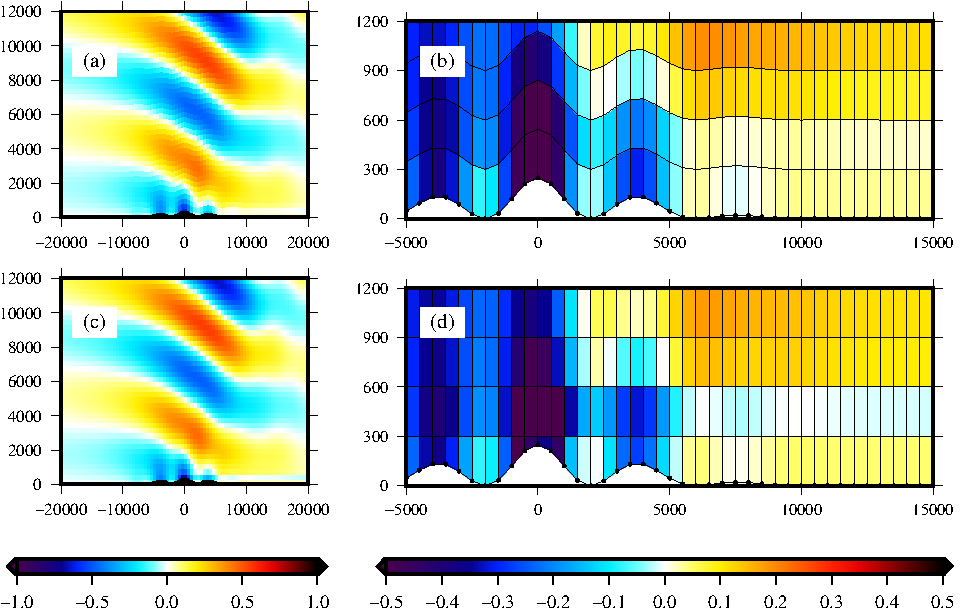
\includegraphics[width=5in]{fig-gravityWaves-theta.pdf}
%
	\caption{Differences in potential temperature in the gravity waves test at the end of the five hour integration.  The centre of the domain is shown on (a) the BTF grid, and (c) the cut cell grid.  Enlargements of the lowest \SI{1200}{\meter} are shown on (b) the BTF grid, and (d) the cut cell grid.  Note that the shorter potential temperature scale is used in the enlargements to reveal the grid-scale oscillation on the cut cell grid.  Figure taken from \citet{shaw-weller2015}.}
	\label{fig:gw-thetaDiff}
\end{figure}

In the gravity waves test, vertical velocities on all grids are in agreement with the high resolution solution from \citet{melvin2010}.  We also compared the difference in potential temperature between the start and end of integration and, overall, the fields were qualitatively similar across all grids.  However, in the lee of the mountain on the cut cell grid, we found that the potential temperature in the lowest layer was anomalously high, and anomalously low in the layer immediately above (figure~\ref{fig:gw-thetaDiff}d).  No such grid-scale oscillation was found in the Exner function of pressure.  This indicates that the Lorenz computational mode has been excited on the cut cell grid.

The model from WS14 uses a Lorenz staggering of variables in which potential temperature, $\theta$, is stored at cell centres and velocities are stored at cell faces.  When calculating vertical momentum at cell faces, $\theta$ must be interpolated from adjacent cell centres.  Any grid-scale oscillation will become invisible to the model and discrete hydrostatic balance will be preserved \citep{arakawa-konor1996}.

\begin{figure}
	\centering
	\documentclass[tikz]{standalone}
\usepackage{bm}
\usetikzlibrary{patterns}
\input{mathmacros}
\input{dissertationmacros}
\begin{document}
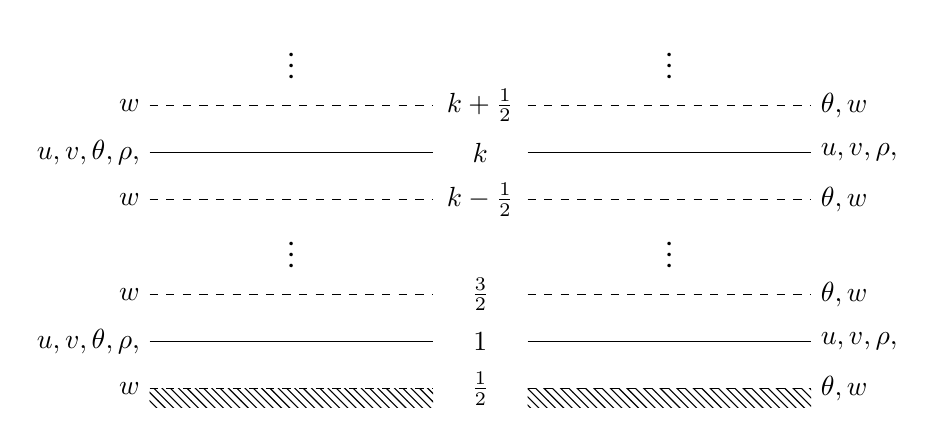
\begin{tikzpicture}[
  scale=0.6
]
\fill [pattern=north west lines] (0,0) rectangle (6,-0.4);
\fill [pattern=north west lines] (8,0) rectangle (14,-0.4);
\node at (7,0) {$\frac{1}{2}$};
\draw [dashed] (0,0) -- (6,0) node [at start, anchor=east] {$w$};
\draw [dashed] (8,0) -- (14,0) node [at end, anchor=west] {$\theta, w$};

\node at (7,1) {$1$};
\draw (0,1) -- (6,1) node [at start, anchor=east] {$u, v, \theta, \rho, \exner$};
\draw (8,1) -- (14,1) node [at end, anchor=west] {$u, v, \rho, \exner$};

\node at (7,2) {$\frac{3}{2}$};
\draw [dashed] (0,2) -- (6,2) node [at start, anchor=east] {$w$};
\draw [dashed] (8,2) -- (14,2) node [at end, anchor=west] {$\theta, w$};

\node at (3,3) {$\vdots$};
\node at (11,3) {$\vdots$};

\node at (7,4) {$k - \frac{1}{2}$};
\draw [dashed] (0,4) -- (6,4) node [at start, anchor=east] {$w$};
\draw [dashed] (8,4) -- (14,4) node [at end, anchor=west] {$\theta, w$};

\node at (7,5) {$k$};
\draw (0,5) -- (6,5) node [at start, anchor=east] {$u, v, \theta, \rho, \exner$};
\draw (8,5) -- (14,5) node [at end, anchor=west] {$u, v, \rho, \exner$};

\node at (7,6) {$k + \frac{1}{2}$};
\draw [dashed] (0,6) -- (6,6) node [at start, anchor=east] {$w$};
\draw [dashed] (8,6) -- (14,6) node [at end, anchor=west] {$\theta, w$};

\node at (3,7) {$\vdots$};
\node at (11,7) {$\vdots$};
\end{tikzpicture}
\end{document}

%
	\caption{Lorenz (left) and Charney--Phillips (right) vertical staggering of variables, in which vertical velocities, $w$, are stored at half levels denoted by dashed lines; horizontal velocities, $u$ and $v$, potential temperature, $\theta$, density, $\rho$, and the Exner function of pressure, $\exner$, are stored at full levels denoted by solid lines.  Adapted from \cite{holdaway2013a}.}
	\label{fig:staggering}
\end{figure}

The Charney--Phillips staggering collocates vertical velocity and potential temperature so that no interpolation is necessary.
Figure~\ref{fig:staggering} illustrates the two arrangements, with solid lines being equivalent to cell centres and dashed lines equivalent to cell faces.}

	\item[Potential temperature advection errors are inconclusive]{In the final test from the Masters dissertation, the initial potential temperature was advected in a prescribed terrain-following flow.  Similar errors were seen on the cut cell grid, but in this test the lowest layer was anomalously low, and the layer above anomalously high.  This result was inconclusive and we have chosen not to pursue this test further.}
\end{description}

\section{Areas of future research}
Recently, I have been considering future directions of my research, based on conclusions from current results and discussions with my supervisors and other researchers:
\begin{description}
	\item[Charney--Phillips staggering on cut cell grids]{Motivated by the errors in potential temperature on the cut cell grid in the gravity waves test, we want to formulate a Charney--Phillips staggering and augment the model from WS14 to allow either staggering to be selected.  We hope that the potential temperature error would be removed by this modification.  We should further motivate this work by varying parameters in the gravity waves test in an attempt to create larger magnitude grid-scale $\theta$ errors.  This is an area in which Hilary is already experienced, and this work will give me a deeper understanding of how the model is constructed.}

	\item[TF/cut cell blended grid]{TF suffer from larger horizontal pressure gradient errors near steep mountains, while cut cells have poor resolution above high mountains.  By combining the two techniques we could formulate a grid which performs well over high mountains and near steep mountains.  Similar grids have been constructed for ocean modelling \citep{burchard-petersen1997,barron2006}, but we are not aware of such techniques being applied in atmospheric models.} 
	\item[3D tests]{We could extend our investigation of TF and cut cell grids into 3D in order to investigate flow blocking regimes.  This would complement the work on TF/cut cell blended grid, offering further verification of the new technique.}

	\item[Large scale tests with Coriolis forces]{To verify the model in large scale flows we could construct tests with an $f\text{-plane}$ or $\beta$-plane approximation, or apply the model on a sphere.  Once again, such tests would help verify the efficacy of a TF/cut cell blended grid.}

	\item[Mass coordinates and moving meshes]{Mike Cullen has spoken with us about the difficulties associated with the upper boundary condition, wave reflections, and sponge layers.  We could investigate extending the model to use mass coordinates by using moving meshes.  The exact nature of this work is uncertain and would require further discussions with Mike Cullen.}

	\item[Understand connection to parametrizations]{Since my work focuses on the dynamical core, I feel it is important to understand how both resolved and unresolved orography are treated in numerical models.  To this end, I have spoken to Miguel Teixeira for suggested reading material relating to drag parametrization.  It might be valuable to spend a small amount of time collaborating with other PhD students who are already working on parametrized orography, although I am uncertain what form such collaborative work might take.}

	\item[Consider roughness/drag forces]{Terry Davies has spoken to me about his ideas for calculating roughness/drag magnitudes by considering the surrounding terrain on the grid.  Further discussions with Terry would be required to progress this work.}
\end{description}

\section{Training and development}
As of June 2015, I have presented at one conference and taken one taught module, as well as giving a number of presentations at university.

\subsection{Taught modules}
In autumn term 2014, I was enrolled in three modules:
\begin{itemize}
	\item MA3NA2 Numerical Analysis II
	\item MAMCDE Partial Differential Equations
	\item MAMB10 Theory and Techniques of Data Assimilation
\end{itemize}
Due to my suspension I was unable to complete these modules, and I hope to take them in autumn term 2015.

In spring term 2015, I obtained 78\% in MAMNSP Numerical Solution of Partial Differential Equations.  The course covered finite difference, finite volume and finite element methods.  It focused on elliptic boundary value problems, stability analysis and error analysis.  The course has already proved useful, and I used the lecture material to understand how to implicitly solve the Poisson equation that appears in Chorin's projection method.

I also intended to study M5MA47 Finite Elements this spring, but chose to drop this module because I lacked the necessary prerequisites.  Now that I have covered an introduction to finite elements in MAMNSP, I would like to enrol in M5MA47 next year if possible.

\subsection{Training}
I have attended three RRDP courses:
\begin{itemize}
	\item How to write a paper
	\item How to write a literature review
	\item How to avoid plagiarism
\end{itemize}
I am also attending the `ECMWF Advanced Numerical Methods for Earth-System modelling' course in June 2015, at which I will also present a poster.

\subsection{Conferences and presentations}
I attended my first conference, `Galerkin methods with applications in weather and climate forecasting', in March 2015, and gave a presentation of my research to date.  Many of the topics were previously unknown to me, and I found it valuable to discover the various numerical techniques that are being developed.

I have presented at university on several occasions at PhD group and Hoskins Half Hour.  I also gave a live demonstration of \texttt{git} and \texttt{make} software in a lunchtime seminar.

I have presented a poster at the Mathematics for Planet Earth (MPE) Jamboree 2014 and at the Met Office Academic Partnership event.  I found that the feedback I received from poster presentations has been useful in guiding my research and study.

I will be attending the SCENARIO Doctoral Training Programme conference and Hoskins@70 event in June 2015.

\subsection{Side projects}
I have spent a small amount of time learning and applying techniques that are related to my research.  These projects are ongoing and I return to them occasionally:
\begin{description}
	\item[Mathematical equivalence of TF coordinates and FV grids]{Many models implement terrain following layers using a coordinate transformation that results in a rectangular computational domain.  However, the finite volume model we have used operates in Cartesian coordinates.  I have worked through some mathematics that begins to show how the two approaches are equivalent for a simplified advection test case with centred differencing.  I have also called upon some of the researchers I met at the Galerkin methods conference to help me with this investigation.  It is not yet clear whether the equivalence holds for higher order methods or other equation sets.}
	\item[Timestepping methods]{In section~\ref{sec:progress} I needed to implement a Runge--Kutta timestepping scheme.  Before describing the scheme in \citet{shaw-weller2015}, I spent an afternoon writing some code to implement Euler's method, Heun's method and the Runge--Kutta scheme so that I could understand the method applied to equations without derivatives.  I could extend this work to ODEs such as a simple harmonic oscillator and investigate numerical stability.}
	\item[Discrete div and curl operators]{Wanting to learn more about primal and dual meshes, I took some of the ideas from \citet{nicolaides1992} in which div and curl are calculated on triangular grids.  I adapted this for an Arakawa C grid, wrote a short program to perform the vector calculus on 2D scalar fields, then gave an interactive presentation about my work at PhD group.  I would like to investigate more of the techniques from \citet{nicolaides1992} so that I can understand Hodge operators and how they are applied to covariant and contravariant velocity fields in WS14.}
\end{description}

\subsection{Teaching}
Shortly before the start of autumn term 2014 I designed and delivered a new three-day training course on Python and Linux programming for the new MPE cohort.  The course covered programming syntax and included practical exercises on numerical approximations, graph plotting and GIS tools.  I hugely enjoyed delivering this course and received positive feedback from the students.  I am keen to seek more teaching opportunities in the future.

This term I am cosupervising Hilary's Masters student, Yumeng Chen, who is working on combining the operator-splitting advection scheme from \citet{leonard1996} with the piecewise parabolic interpolation described by \citet{colella-woodward1984}.  I have assisted in reviewing Yumeng's written work and we hope to collaborate on the tracer advection test over orography from \citet{schaer2002}, comparing his results with those from \citet{shaw-weller2015}.

I am also involved in outreach events.  At the Brighton Science Festival, I played educational games with young children using water and an infrared camera to write invisible messages, and talked to them about today's weather and how it related to seasonal weather.  I hope to attend another science festival with Antonio Portas in June 2015.

\bibliographystyle{ametsoc2014}                                                 
\bibliography{references}

\end{document}
